\chapter{Asking Wealthy Americans How They Got Rich!}

We begin, as the lecture begins, with an effect before we are shown its causes. A large exit appears first, Miami is then used as a field of comparison, and only after several smaller but very concrete cases do we return to Ann Malum for the longer argument. The mathematical content here is necessarily modest and editorial. Still, there is a real quantitative spine beneath the conversation: ownership, repeatable cash flow, scalable operating systems, capital structure, leverage, and compounding. The lecture is not asking us to admire wealth from a distance; it is asking us to trace the mechanisms by which wealth is built, preserved, and then made productive again.

\section{The Sale Before the System}

The opening move is simple and powerful. The host does not begin with a theory of entrepreneurship. He begins with a founder who sold a company and realized a large personal outcome. Ann Malum reports that her own equity shares were worth about \$90 million, while the company itself was valued at a little over \$300 million. This gives us, immediately, the distinction between enterprise value and realized founder wealth.

We write the opening data as
\begin{equation}
E_{\mathrm{Ann}} \approx \$90\,\mathrm{M},
\qquad
V_{\mathrm{company}} \gtrsim \$300\,\mathrm{M}.
\end{equation}
The lecture does not ask for a cap-table reconstruction, but the numbers invite a quick estimate of implied ownership:
\begin{equation}
s_{\mathrm{Ann}} \approx \frac{E_{\mathrm{Ann}}}{V_{\mathrm{company}}} \approx 0.30.
\end{equation}
This should be stated carefully. It is only rough arithmetic from spoken figures, not an audited statement of ownership. Still, it does what the lecture wants done at the beginning: it separates the founder's realized slice from the larger value of the company itself.

There is also an important correction to the host's tone. The opening can sound, for a moment, like a story about one sudden day. But when Ann later reflects on the sale, she insists that the wire came in a day while the value was created over nine and a half years. So the chapter should keep both timescales in view: the payout is instantaneous, the building is not.

\subsection{A Worked Estimate}

The lecture does not derive the implied ownership share explicitly, but the estimate is worth preserving because it sets the scale of the whole discussion.

\begin{enumerate}
\item Take the stated personal equity outcome \(E_{\mathrm{Ann}} \approx \$90\,\mathrm{M}\).
\item Take the stated company value \(V_{\mathrm{company}} \gtrsim \$300\,\mathrm{M}\).
\item Form the quotient \(s_{\mathrm{Ann}} = E_{\mathrm{Ann}}/V_{\mathrm{company}}\).
\item Obtain the rough estimate \(s_{\mathrm{Ann}} \approx 0.30\).
\item Record the result only as a back-of-the-envelope ownership fraction.
\end{enumerate}

This is the lecture's first quiet lesson. Wealth at the surface is spectacle; underneath it lies allocation.

\section{A Field of Cases: Pressure, Motion, and Brand}

The lecture now delays the promised mansion interview and goes out into Miami. This is not filler. The host turns the city into a comparative lab. We are shown not one route to wealth, but several distinct machines.

The first entrepreneur gives the most pressure-driven account. She leaves Saudi Arabia at eighteen, loses family financial support when her father's business fails, works multiple jobs, and describes that period not merely as hardship, but as compulsion: when there is no way out, one makes a way. The lecture wants this account early because it establishes a recurring motif of the whole chapter: pressure is not presented as pleasant, but it is repeatedly presented as clarifying.

Her later business claim is concrete:
\begin{equation}
R_{\mathrm{young}} \approx \$20\,\mathrm{M}/\mathrm{yr},
\end{equation}
with the explicit caveat that this is the business figure for her and her partners, not a stated personal draw.

From that biography the lecture pivots to an operating rule. She says, in effect, that the smartest people often stall because they overanalyze, while the people who move faster discover the missing steps only after acting. We may summarize the contrast as
\begin{equation}
\text{speed} > \text{perfectionism}.
\end{equation}
This is not a theorem, but it is an accurate compression of the logic in her interview. The market rewards learning-by-doing more than immaculate premeditation.

\subsection{Question \& Answer}

\paragraph{Question.} Do we need the whole plan before we move?

\paragraph{Answer.} The lecture's answer is no. We are urged to see action itself as an information-generating process. The missing parts of the plan do not always yield to reflection. Often they appear only after contact with the world. What looks, from the outside, like boldness is treated here as a practical way of discovering what cannot be known in advance.

The interview then changes register once more. We move from adversity into the mechanics of visibility. On social media, she says, people are not generous with attention; they do not give many second chances. So the first three seconds become decisive:
\begin{equation}
t_{\mathrm{hook}} = 3\,\mathrm{s}.
\end{equation}
From there the lecture gives us a branding funnel that is worth writing cleanly:
\begin{equation}
\text{hook} \to \text{attention} \to \text{perspective shift} \to \text{respect} \to \text{pricing power}.
\end{equation}
The hook wins a hearing. The perspective shift gives a reason to continue. Respect then becomes the bridge between visibility and commerce. This is why the interview links sales and branding so tightly: brand is treated not as ornament, but as a machine for attracting opportunities.

\begin{figure}[h]
\centering
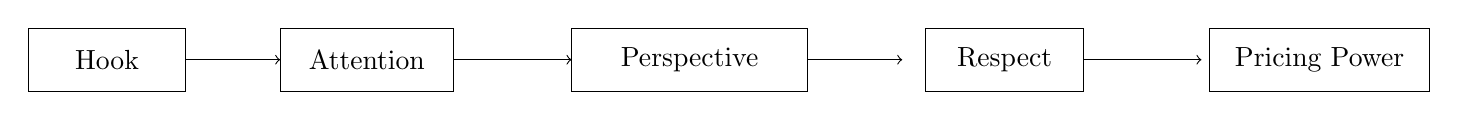
\begin{tikzpicture}
\node[draw, rectangle, minimum width=2.0cm, minimum height=0.8cm] (a) at (0,0) {Hook};
\node[draw, rectangle, minimum width=2.2cm, minimum height=0.8cm] (b) at (3.3,0) {Attention};
\node[draw, rectangle, minimum width=3.0cm, minimum height=0.8cm] (c) at (7.4,0) {Perspective};
\node[draw, rectangle, minimum width=2.0cm, minimum height=0.8cm] (d) at (11.4,0) {Respect};
\node[draw, rectangle, minimum width=2.8cm, minimum height=0.8cm] (e) at (15.4,0) {Pricing Power};
\draw[->] (1.0,0) -- (2.2,0);
\draw[->] (4.4,0) -- (5.9,0);
\draw[->] (8.9,0) -- (10.1,0);
\draw[->] (12.4,0) -- (13.9,0);
\end{tikzpicture}
\caption{A transcript-derived branding funnel. The lecture's claim is that a short attention window, if used well, can be converted into respect and then into commercial leverage.}
\end{figure}

So the first field case gives us two linked doctrines. Under pressure we move, and in public we must learn to make that movement legible.

\section{Recurring Revenue, Systems, and the Buy-Don't-Start Lane}

The second interview changes the grammar of the lecture. We move away from social-media brand and into repeatable business architecture. The speaker owns a large tanning-salon franchise network and claims a net worth above \$100 million. The business sounds ordinary; that is precisely the point. The lecture now wants to show that glamour at the level of outcome may rest on something very unglamorous at the level of cash flow.

The core concept is recurring revenue. We may represent the stream of repeat payments as
\begin{equation}
R_{\mathrm{rec}} = \sum_{t=1}^{T} r_t,
\end{equation}
where \(r_t\) is the payment received in period \(t\). This schematic is simple, but it captures the lecture's point exactly. A one-off sale is finite. A system that reliably produces \(r_1,r_2,\dots,r_T\) is much closer to a wealth machine.

The same interview gives concrete scale markers:
\begin{equation}
N_{\mathrm{tan}} \approx 270,
\qquad
W_{\mathrm{tan}} > \$100\,\mathrm{M}.
\end{equation}
It then adds a second principle: one should build systems early enough that the business can be replicated. That is the point of the cited idea of acting as if one had \(500\) locations even when one had one. In notation,
\begin{equation}
S_1 \rightsquigarrow S_{500},
\end{equation}
where \(S_n\) denotes an operating system that remains valid as scale changes.

\subsection{Question \& Answer}

\paragraph{Question.} Can we buy a real business even if we do not have much money?

\paragraph{Answer.} The lecture answers yes, but only after it gives the surrounding market condition. We are told that many older owners want to retire, that their children often do not want the business, and that there are more businesses for sale than there are willing buyers. The imbalance may be written as
\begin{equation}
B_{\mathrm{sale}} > B_{\mathrm{buyers}}.
\end{equation}
That imbalance opens the door to owner financing. In a minimal schematic,
\begin{equation}
P = D + F_{\mathrm{seller}},
\end{equation}
where \(P\) is the purchase price, \(D\) the buyer's down payment, and \(F_{\mathrm{seller}}\) the seller-carried note.

The lecture's claim is therefore not that capital is unnecessary. It is that the structure of capital can change when the seller needs an exit more than the market supplies a buyer. This is why the lecture steers us toward boring businesses. The absence of glamour is not a weakness; it is part of the opportunity.

The interview also makes a brief but useful detour into AI. The point is not that AI abolishes work. Rather, it changes the headcount needed to run a department. If the old requirement was \(50\) people, the new requirement may be smaller:
\begin{equation}
L_{\mathrm{after\ AI}} < 50.
\end{equation}
The transcript does not preserve the missing number, so we should not invent it. Still, the lecture clearly wants to preserve the broader thought: tools alter operating leverage.

\section{Industrial Real Estate and the Capital Question}

The third major field case comes from real estate, and with it the lecture acquires a different rhythm. The speaker is not selling a personal brand and not describing a subscription business. He is describing demand, timing, and risk. Industrial real estate is introduced through a chain of practical causation:
\begin{equation}
\text{COVID e-commerce} \to \text{warehouses/distribution centers} \to \text{industrial demand}.
\end{equation}
What matters here is the method of argument. The lecture does not begin with a valuation model. It begins with packages arriving at houses and asks where those packages come from.

The financial anchor is again large and concrete:
\begin{equation}
V_{\mathrm{devco}} \gtrsim \$4\,\mathrm{B}.
\end{equation}
This number, too, is not used for detailed calculation. It is used to demonstrate what can happen when industry timing and aggressive risk-taking align.

\subsection{Question \& Answer}

\paragraph{Question.} Do we actually need a lot of money to get into real estate?

\paragraph{Answer.} The lecture says no, provided we hear the sentence correctly. It does not mean that capital no longer matters. It means that initial cash in the operator's pocket is not the only form capital can take. Trust, track record, and aligned investors are also part of the capital structure. In the lecture's own rhythm, one first states the objection, then dissolves it: we need people who believe in the operator, share the vision, and stand to make money from the project.

The logic can be compressed as
\begin{equation}
\text{vision} + \text{credibility} \to \text{investor backing}.
\end{equation}
The lecture then pushes further into Miami itself and makes a second causal claim about multi-residential real estate:
\begin{equation}
\text{lower liquidity} \to \text{shift from owning to renting}.
\end{equation}
This is a useful reminder that the lecture is always trying to move from a balance-sheet condition to a business consequence. Reduced household liquidity becomes rental demand.

\begin{figure}[h]
\centering
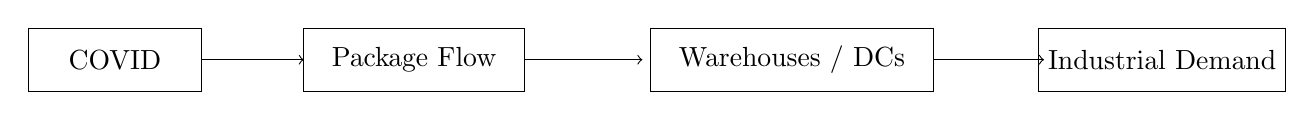
\begin{tikzpicture}
\node[draw, rectangle, minimum width=2.2cm, minimum height=0.8cm] (a) at (0,0) {COVID};
\node[draw, rectangle, minimum width=2.8cm, minimum height=0.8cm] (b) at (3.8,0) {Package Flow};
\node[draw, rectangle, minimum width=3.6cm, minimum height=0.8cm] (c) at (8.6,0) {Warehouses / DCs};
\node[draw, rectangle, minimum width=3.0cm, minimum height=0.8cm] (d) at (13.3,0) {Industrial Demand};
\draw[->] (1.1,0) -- (2.4,0);
\draw[->] (5.2,0) -- (6.7,0);
\draw[->] (10.4,0) -- (11.8,0);
\end{tikzpicture}
\caption{A transcript-derived industrial-demand chain. The lecture motivates the asset class by logistics first and only afterward by scale.}
\end{figure}

At this point the Miami fieldwork has done its job. We have seen pressure, brand, recurring revenue, boring-business acquisition, and industrial timing. Only now is the lecture ready to return to Ann Malum.

\section{Ann Malum: A Category, a Loop, and a North Star}

When the lecture arrives at Ann Malum's house, it does not immediately begin with tactics. Instead it returns once more to the sale day. That is a good sign. The lecture refuses to let the wire transfer detach from the years that created it. Ann says the moment felt real because she knew the value she had built. This restores continuity between the opening spectacle and the longer operating story.

That story begins with category discovery. Ann says, in effect, that she succeeded by finding things before the market had fully found them. The Solidcore case is not presented as a generic fitness success. It is presented as the recognition of something not yet properly named. The workout was not exactly Pilates and not exactly strength training. So the business needed language before it needed scale.

The lecture's most important growth claim in this section is that Solidcore spent nothing on paid marketing for its first four years:
\begin{equation}
M_{\mathrm{paid}} = 0
\qquad
\text{for the first }4\text{ years.}
\end{equation}
Why did that work? Because the product created a story that customers themselves wanted to carry. The growth loop can be written
\begin{equation}
\text{workout novelty} \to \text{soreness} \to \text{retelling} \to \text{new users}.
\end{equation}
This is one of the lecture's best moments. A category that initially suffers from lack of language becomes a category that generates its own language through user experience.

\subsection{Question \& Answer}

\paragraph{Question.} Why did Solidcore grow for years without paid marketing?

\paragraph{Answer.} Because the product itself supplied the evidence. The workout was unusual enough to be memorable and hard enough to be retold. That changed customers into narrators. In such a case the absence of paid marketing does not mean the absence of marketing. It means that the transmission channel is social rather than purchased.

The next piece of structure is the North Star. Ann says that from the beginning she knew the destination:
\begin{equation}
N_{\mathrm{target}} = 100.
\end{equation}
This matters because it explains a line in the transcript that might otherwise sound like mere bravado: when franchising opportunities or early buyout offers appeared, she did not experience them as obvious wins. Measured against a plan aimed at \(100\) studios, they were intermediate branches that threatened to dilute the line of motion.

There is also a more interior argument in this section. Ann says that not everybody is built for entrepreneurship, and she grounds the claim not in mystique but in fit. The right business must match a real personal edge. We may represent that heuristic as
\begin{equation}
q_{\mathrm{edge}} > q_{0.95},
\end{equation}
meaning that one should identify what one does better than roughly \(95\%\) of the population and attach that edge to a business that needs precisely that capability. The notation is editorial, but the principle is one of the lecture's closing selection rules.

\section{After the Exit: Public Equities, Leverage, Compounding, and Negotiation}

The lecture's last movement is also its most explicitly financial. Ann shifts from building a company to handling wealth after the exit. She says she is in wealth-preservation mode, though still with meaningful risk tolerance. The first summary of her balance sheet is simple:
\begin{equation}
w_{\mathrm{public}} \approx 0.50,
\qquad
H_{\mathrm{NVDA}} > \$10\,\mathrm{M}.
\end{equation}
She then adds a speculative AI-market remark: some people, she says, imagine Nvidia around \$800 by 2030 against a present price near \$152. The chapter should preserve this not as a valuation result, but as evidence of how she is framing the AI opportunity set.

The lecture's clearest financial distinction between rich and wealthy appears next. Once one has a sufficiently large asset base, one may borrow against assets rather than liquidate them. The rough borrowing structure is given as
\begin{equation}
L_{\mathrm{credit}} \approx \$50\,\mathrm{M},
\qquad
r_m \approx 5\%,
\qquad
t_{\mathrm{cg}} \approx 20\%.
\end{equation}
The transcript is noisy at one point, but the intended comparison is stable: selling appreciated stock costs around \(20\%\) in capital-gains tax, while borrowing against the portfolio costs around \(5\%\).

\subsection{Question \& Answer}

\paragraph{Question.} Why would a wealthy person borrow against stock instead of selling it?

\paragraph{Answer.} Because the relevant comparison is not between borrowing and doing nothing. It is between the cost of borrowing and the cost of liquidation. The lecture's implicit balance looks like this:
\begin{align}
\text{cost of selling} &\sim t_{\mathrm{cg}} \approx 20\%,\\
\text{cost of borrowing} &\sim r_m \approx 5\%.
\end{align}
So if the next opportunity offers return \(r_i\), and if
\begin{equation}
r_i > r_m,
\end{equation}
then borrowing may dominate selling on the lecture's own logic. Ann's examples are loans or private investments yielding double digits:
\begin{equation}
r_i \in [12\%,15\%].
\end{equation}
This is the spread the lecture wants us to see.

\subsection{A Worked Capital Comparison}

We may write the borrow-versus-sell argument step by step.

\begin{enumerate}
\item Suppose capital is needed for a new investment.
\item Selling appreciated stock realizes gains and costs about \(t_{\mathrm{cg}} \approx 20\%\).
\item Borrowing against the portfolio costs about \(r_m \approx 5\%\).
\item If the opportunity offers \(r_i \in [12\%,15\%]\), then \(r_i > r_m\).
\item On the lecture's logic, borrowing preserves the original asset base, avoids immediate realization of gains, and still permits new deployment of capital.
\end{enumerate}

The lecture then broadens from leverage to compounding. Ann gives a low point and a recovery point in her public-equity account:
\begin{equation}
W_{\mathrm{low}} \approx \$39\,\mathrm{M},
\qquad
W_{\mathrm{later}} \approx \$64\,\mathrm{M},
\qquad
\Delta W_{\mathrm{day}} \approx \$1.2\,\mathrm{M}.
\end{equation}
The qualitative law behind the passage is standard:
\begin{equation}
W_{t+1} = (1+r_t)W_t.
\end{equation}
Nothing here depends on a single fixed return. The lecture's point is instead that wealth behaves differently once the base is large enough: fluctuations measured in millions can occur without labor input that day, simply because the asset base is already at work.

\begin{figure}[h]
\centering

\begin{tikzpicture}
\node[draw, rectangle, minimum width=3.0cm, minimum height=0.8cm] (a) at (0,0) {Public Equities};
\node[draw, rectangle, minimum width=3.2cm, minimum height=0.8cm] (b) at (4.8,0) {Credit Line};
\node[draw, rectangle, minimum width=3.6cm, minimum height=0.8cm] (c) at (10.3,0) {New Investment};
\node[draw, rectangle, minimum width=2.8cm, minimum height=0.8cm] (d) at (15.2,0) {Return Spread};
\draw[->] (1.5,0) -- (3.2,0);
\draw[->] (6.4,0) -- (8.0,0);
\draw[->] (12.1,0) -- (13.8,0);
\end{tikzpicture}
\caption{A transcript-derived leverage chain. The lecture's financial point is that a large asset base can be used as collateral for new deployment without immediate liquidation.}
\end{figure}

The final financial contrast is deliberately blunt:
\begin{equation}
r_{\mathrm{bank}} < 0.5\%.
\end{equation}
The chapter should preserve the tone without turning it into doctrine. The lecture is not proving a universal theorem about banking. It is making a practical complaint: money left inert in a low-yield account does not participate in the compounding game.

The section ends, appropriately, not with a market formula but with negotiation. Ann says that one must make the other party like and believe in the operator. The chapter should keep one concrete marker from that discussion, namely the later example of roughly six months of free rent:
\begin{equation}
F_{\mathrm{rent\ concession}} \approx 6\,\mathrm{months}.
\end{equation}
That number is small compared to the portfolio figures, but its function is important. It reminds us that wealth in the lecture is not only an outcome of capital allocation; it is also repeatedly an outcome of persuasion.

\section{Summary}

The lecture opens with wealth as event and closes with wealth as system. Along the way we are shown several distinct engines: adversity turned into motion, attention turned into pricing power, recurring payments turned into business stability, retiring owners turned into acquisition opportunity, logistics turned into industrial demand, category confusion turned into word-of-mouth growth, and finally a large asset base turned into leverage and compounding.

What gives the lecture its shape is that it never treats these as disconnected tricks. They are successive answers to one question: how does a visible outcome arise from an invisible structure? By the end the answer is sharper. Wealth is not merely income at higher scale. It is the result of building value, keeping the line of growth clear, learning the rules of capital, and then allowing the accumulated base to work on its own behalf.